\input{wsc15style.tex}     % download from author kit.  Style files for wsc formatting. Don't remove this line - required for generating the final paper!

\documentclass{wscpaperproc}
\usepackage{latexsym}
\usepackage{caption}
\usepackage{graphicx}
\usepackage{mathptmx}
\usepackage[utf8]{inputenc}


%****************************************************************************
%% AUTHOR: You may want to use some of these packages. (Optional)
%\usepackage{amsmath}
%\usepackage{amsfonts}
%\usepackage{amssymb}
%\usepackage{amsbsy}
%\usepackage{amsthm}

\usepackage{algorithm,algorithmicx,algpseudocode}
\usepackage{float}
\usepackage{booktabs}
 \usepackage{multirow}


\algnewcommand\And{\textbf{and}}

\usepackage{mathtools}
\DeclarePairedDelimiter\abs{\lvert}{\rvert}%
\DeclarePairedDelimiter\norm{\lVert}{\rVert}%

\newcommand{\specialcell}[2][c]{%
  \begin{tabular}[#1]{@{}c@{}}#2\end{tabular}}


\makeatletter
\let\oldabs\abs
\def\abs{\@ifstar{\oldabs}{\oldabs*}}
\let\oldnorm\norm
\def\norm{\@ifstar{\oldnorm}{\oldnorm*}}
\makeatother

\usepackage{xcolor}
    \usepackage{cite}


\newcommand{\memo}[2]{\textcolor{#1}{#2}}
\newcommand{\added}[2]{\textcolor{#1}{#2}}
%\renewcommand{\memo}[2]{} % uncomment in the final version
%\renewcommand{\added}[2]{#2} % uncomment in the final version
\newcommand{\todo}[1]{\memo{red}{TODO: #1\\}}
\newcommand{\simon}[1]{\memo{green}{Simon: #1\\}}
\newcommand{\jm}[1]{\memo{blue}{JM: #1\\}}
\newcommand{\xrc}[1]{\memo{orange}{XRC: #1\\}}
\newcommand{\new}[1]{\added{orange}{#1}}

\begin{document}

\WSCpagesetup{Montanier, Carrignon and Rubio}

\title{Modelling the Co-evolution of Trade and Culture in Past Societies}

\maketitle

\begin{figure*}[htb]
{
\centering
Jean-Marc Montanier\\
Simon Carrignon\\ 
Xavier Rubio-Campillo\\
\vspace{12pt}
Barcelona Supercomputing Center\\
Carrer de Jordi Girona, 29, \\
08034 Barcelona, Spain\\
}
\end{figure*}


\section*{ABSTRACT}

This papers presents a new framework to study the co-evolution of cultural transmission and trade. The design aims for a trade-off between the flexibility necessary for the implementation of multiple models and the structure necessary for the comparison between the models implemented. To create this framework we propose an Agent-Based Model relying on agents producing, exchanging and associating values to a list of goods. We first present the key concepts of the framework and two examples of its implementation which allow us to show the flexibility of our framework. We then compare the results obtained by the two models, thus validating the structure of the framework. Finally, to validate our trading model we study the price structure obtained.


\section{INTRODUCTION}\label{sec:intro}

% the spread of cultural traits is often modelled following neutral theory

Cultural change comprises the collection of processes that promotes or inhibits the spread of information by social interaction within a population~\cite{boyd_origin_2005}. An increasing number of social scientists are using an evolutionary framework to model these dynamics, thus fostering the development of transdisciplinary efforts designed to understand cultural evolution~\cite{henrich_evolution_2003}.

Several studies focus on the biases that affect the transmission of cultural traits, including the relevance of intrinsic traits and frequency dependence properties. These analysis often compare evidences against neutral models~\cite{neiman_stylistic_1995}. They assume that traits do not affect the fitness of the individual that acquires it; within this context its transmission is unbiased, and its success will depend on its popularity amongst the rest of individuals. This neutral model generates a distinctive pattern of frequency distribution of traits, identified as a power law. It can be replicated with a simple random copying transmission mechanism~\cite{bentley_random_2004}: an individual will copy the traits of a randomly chosen individual with a given probability. This copy can potentially introduce some errors in the acquired trait, which account for innovation processes. The individual will in turn continue to spread these cultural traits which will be further adopted by other individuals. This basic model can be enriched by several additional processes both in the innovation~\shortcite{schillinger_copying_2014,sole_evolutionary_2013,ziman_technological_2003} and the transmission~\cite{heyes_social_1994,henrich_evolution_2003}. Unbiased transmission works as a baseline for identifying frequency-dependent biases: if evidence has higher tendency to copy the most common trait is is known as conformism, while the opposite is defined as anti-conformism.

This approach can be used as the starting point to analyse patterns of cultural change to explore frequency-dependance in archaeological contexts~\cite{lipo_neutralitystyle_2001,shennan_ceramic_2001,steele_ceramic_2010}. However, the fact that archaeology records fragmented material culture presents some challenges on the validity of the method~\cite{kandler_nonequilibrium_2013,porcic_exploring_2014,crema_approximate_2014}.

This work explores the impact of a crucial element on the transmission of material culture: trade. Networks of good exchanges are being increasingly recognised as key elements that structured ancient societies~\shortcite{temin_market_2001,remesal_epnet_2014,brughmans_connecting_2010}. The scenarios where this process emerge suggest a complex bias in the selection of cultural traits, which at the same time are also identified as economic goods~\cite{bentley_specialisation_2005,macmillan_agent-based_2008}. Trasmission is not neutral anymore, as different prices for each good will introduce a dynamic content bias. This affects the frequency of the good within the population, which in turn would modifies its price following a co-evolutionary dynamic.

This work explores these co-evolutionary dynamics using a theoretical Agent-Based Model (ABM), a type of simulation particularly useful for studying non-linear dynamics in heterogeneous environments within an evolutionary perspective~\cite{lake_trends_2014}. Next section defines the model, which is based on unbiased transmission mechanisms and simple exchange dynamics. Next, we define different experiments to explore the dynamics of the created model. Finally, the concluding remarks interpret the results and discuss further possibilities of the pesented model.

\section{MODEL DESCRIPTION}

To explore the co-evolution between trade and cultural change we have developed an ABM where the different agents produce and trade goods to which they associate variable values. The model is composed of a population $Pop$ of $m$ agents, each defined by 2 vectors of size $n$. The first corresponds to the quantity of each good that the agent $i$ possesses: 
$$\forall i \in Pop, \quad Q^i = (q^i_1,\cdots,q^i_n) $$
where $Q^i$ is the total list of possessions of agent $i$, and $q^i_j$ is the number of goods of type $j$ that agent $i$ posses.

The second vector reflects the estimation of the value of a good that an agent $i$ makes.
$$\forall i \in Pop, \quad V^i = (v^i_1,\cdots,v^i_n) $$
where $V^i$ is the total list of estimated values of agent $i$, and $v^i_j$ is the value that agent $i$ associates to the goods of type $j$.

On top of these elements four processes are used: \emph{production}, \emph{cultural transmission}, \emph{innovation} and \emph{trade}. The \emph{production} process describes the creation of goods by the agent. Once a good is produced by an agent $i$ it is added to its quantity vector ($Q^i$). The \emph{trade} process models the exchange of goods between the agents which results in a modification of the quantity vectors ($Q^i$). The amount of goods exchanged is computed by the agents concerned by the trade, within the \emph{trade} process, based on their value vectors ($V^i$). Within the \emph{cultural transmission} process an agent $i$ can copy the value vector ($V^j$) of an agent $j$, where $j \neq i$. Finally, the \textit{innovation} process also modifies the value vector $V^i$ of an agent, but it differs from the \emph{cultural transmission} process in that the modification is done without reference to the other agents.

The scheduling of the four processes is described in algorithm~\ref{algo:complete} along with the vectors modified by each of these processes. Between line 2 and 7 all agents of the population are initialised with empty quantity vectors and random values. Between the lines 11 and 19 is presented the part of the pseudo-code describing the instructions that will be repeated for each iteration of the simulation. One can note that the \emph{trade} process is called at each iteration while the \emph{cultural transmission} and \emph{innovation} processes are executed only every $CulturalStep$. The idea behind this is to perform the \emph{cultural transmission} based on a score that reflects the performance of the agent and not only one lucky or unlucky trading round. The timestep number used in the figures of this article refers to the number of times the \emph{cultural transmission} and \emph{innovation} processes are called.

\begin{algorithm}
\caption{Model}
\label{algo:complete}
	\begin{algorithmic}[1]
	\scriptsize
	\State INITIALIZATION: 
		\For{$j \in Goods$}
			\For{$i \in \#Pop/\#Goods$} \Comment{Initialize the agent with no goods and a random value vector}
				\State $Q^i = (0, \cdots, 0)$
				\State $V^i = (v^i_0, \cdots, v^i_n)$ \Comment{The values of $v^i_j$ are selected randomly}
			\EndFor
		\EndFor

	\State SIMULATION:
		\Loop{$~step \in TimeSteps$}
			\For{$i \in Pop$}
				\State $Production(Q^i)$
				\For{$j \in Pop$}
					\State $TradeProcess(V^i,Q^i,V^j,Q^j)$
				\EndFor				
				\If{$ (step \mod CulturalStep) = 0$}	
					\State $CulturalTransmission(V)$
					\State $Innovation(V^i)$
				\EndIf
			\EndFor
		\EndLoop
\end{algorithmic}
\end{algorithm}


In order to validate our model we first reproduce common results from the literature on cultural transmission. We then show that it is possible to transform our model to fit processes that are economically sound, i.e. the model should show the convergence optimal values such as shown in~\cite{gintis_emergence_2006}. To achieve these two goals, we have design for each one a specific set of implementations of the four core processes (production, trade, cultural transmission and innovation). 

%These dynamics are modelled after processes (production, cultural transmission, innovation and trade) which will be explained in further details later. The flexibility of the models comes from the possibility to implement these processes differently depending on the hypothesis tested. However, since all experiments are performed with the same four processes, the effect of the various implementations of one process can be studied easily. Moreover, the operating of the model revolves around the value that agents associate to goods. Depending on the question studied, the value can reflect the interest of the agent for the good or it can be the price at which the agent evaluate this good. Since this vector is common to all experiments performed with this model, it is extremely useful for the comparisons of results obtained with different implementation of the key processes.

\subsection{Neutral Model}\label{sec:culturalTrans}

The first set of implementations is designed to reproduce a scenario of unbiased transmission, where each good is a cultural trait without intrinsic positive or negative weight \cite{bentley_random_2004,bentley_specialisation_2005,mesoudi_random_2009}. 
Under this hypothesis, the processes of \emph{production} and \emph{trade} are not relevant, and as a consequence, they do not modify the content of the quantity vectors of the agents.
%%simon: I would rather say  something like :
%%Under this hypothesis, the processes of \emph{production} and \emph{trade} are not relevant as their results will not affect in any way the evolution of the system.
%% but we could alos simply remove the sentence?

Unbiased \emph{cultural transmission} is implemented using ``random copy'': each agent has a low probability to pick randomly one agent among all and copy its vector of values. The \emph{innovation} process, termed ``unbounded'', is triggered with a low probability ($\mu$) and draw a new random value to replace an element $v^i_j$. The probabilities to trigger \emph{cultural transmission} and \emph{innovation} are presented with other parameters in table~\ref{tab:parameters}.

The neutral hypothesis states that the ``random copy'' transmission and the ``unbounded'' innovation process used under a fixed population size leads to a distribution of frequency of cultural variants termed \emph{power law}. This distribution is characterized by a small number of very frequent traits and a large number of very rare traits. 
%Since this hypothesis has been verified in previous works implementing similar \emph{imitation} and \emph{innovation} mechanisms, we expect in this work the observation of a similar ``power law' distribution. 
More formally, this distribution is formalised as : $$P(v)=C/v^\alpha $$ where $v$ is the number of time a variant has been repeated, $P(v)$ the probability to find that variant, $C$ a constant, $\alpha$ a variable describing the slope of the curve obtained. We will therefore attempt to fit as well as possible the results obtained with this set of implementations to the ``power law'' distribution by modifying the $\alpha$ parameter.

\subsection{Trading Model}\label{sec:trade}

The second set of implementations of the four processes of the framework aims at producing economical dynamics. We are interested in the exchange of goods between agents in a barter process where each agent can choose its prices of exchange. We want to implement simple processes leading to the convergence of all prices to values acceptable by all agents, i.e. we would like to observe, at the end of an experiment, all the agents using a set of prices which allow them to trade efficiently.

\paragraph{Production}
In this set of implementations, each agent is producing only one type of good. The type of good produced by an agent $i$ is assigned to it at the beginning of the simulation, does not change through the simulation and is referred as $produced^i$. 

\paragraph{Cultural transmission}
Within this set of implementations, the cultural transmission process is not random but biased toward the agents which are the best at trading, and is therefore termed ``success bias''. To achieve this bias, the cultural transmission mechanism used takes into account the value vector of the other agents and relies on two new notions: \emph{need} and \emph{score}. 

The \emph{need} is a quantity of good that each agent tries to obtain. This quantity is different for each good but the need for a good is the same for all agents:
$$ N = (n_1, \cdots, n_r) $$ 

The \emph{score} $s^i_j$ of an agent $i$ reflects the ability of this agent to obtain the quantity of good $j$ it needs. It is maximum when the quantity $q^i_j$ that an agent $i$ own of the good $j$ is equal to the need $n_j$ for the good $j$ and lowers proportionally to the distance between the need vector and the quantity vector.  It is formally computed as follow for agent $i$ and the good $j$:

\begin{equation}\label{eq:score}
s^i_j = \begin{cases}
 s_{max}=1 & \text{if $q^i_j = n_j$}\\
1 -\dfrac{\abs{q^i_j - n_j}}{ \sqrt{\abs{(q^i_j)^2-(n_j)^2}}} & \text{if $q^i_j \neq n_j$}
\end{cases}
\end{equation}


This function ensures that each good has the same weight in the final score (i.e.: managing to get only the right amount of a good with a high ``need'' value will not give a better score to the agent).


\begin{figure}[htp]
	\begin{center}
		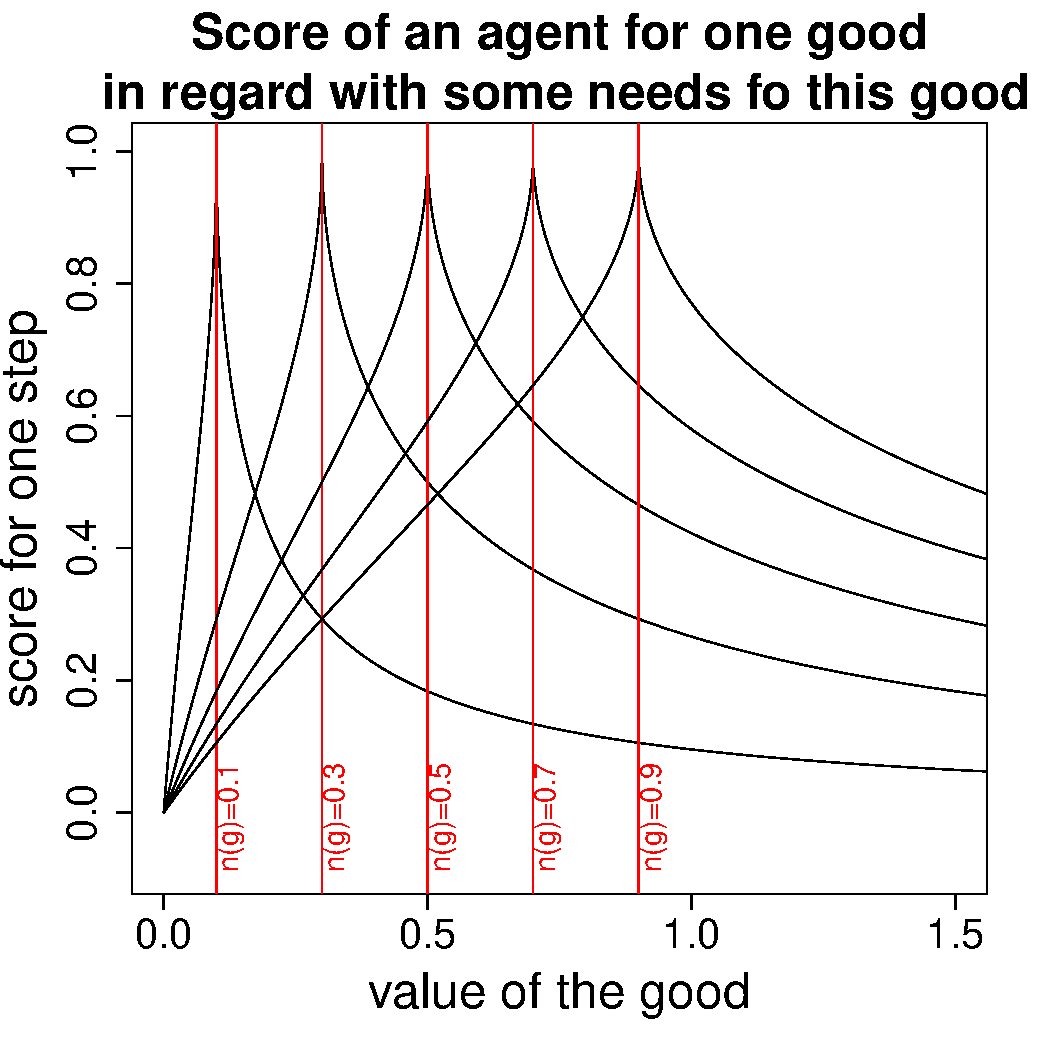
\includegraphics[width=7cm]{img/fitness.pdf}
	\end{center}
	\caption{The payoff depending on the quantity owned of a given good and the effective needs $n(g)$ for this good.}
	\label{fig:fit}
\end{figure}
The figure~\ref{fig:fit} depicts the score of an agent, for different need value of one good, with regards to the quantity of the good possessed by the agent. We can see that even if the need for a good is small (for instance when $n(g) = 0.01$) an agent can have a high score as soon as it manages to get a quantity close to the need. This insures that an agent needs to have for each of the good a quantity equal to the need and that no agent could reach a better score just by getting the right quantity for a good with a high need.

The complete score of an agent $i$ is termed $s^i$ and corresponds to the sum of the $s^i_j$. The agents will choose the agent from whom the price vector should be copied among the agents that produce the same good and have the highest score. In practice, the bottom two percent of the agents (in terms of score) will copy the prices of the top two percent.


\paragraph{Trading} 
During the trading phase the value associated to a good by an agent corresponds to the subjective price of the good for this agent. Briefly summarised, for each good that it does not produce, an agent will trade with the first partner that offers an acceptable trade, i.e. an agent that proposes a satisfiable ratio between the other good and the good produced by the agent. 

In more details, the trading phase starts by the agent looking at a first random agent producing another good. 
Let $o$ be an agent producing $g$ who proposes a trade and $r$ an agent producing $k$ that receives the proposition. As explained earlier, each has a quantity of good $Q^o$ and $Q^r$. On the one side, $o$ wants to exchange a quantity $w_g^o$ of the good $g$ for a quantity $w_k^o$ of the good $k$. On the other side, $r$ wants to exchange a quantity $w_g^r$ of the good $g$ for a quantity $w_k^r$. The tuples $W^o$ and $W^r$ describe the quantities of goods wanted by agent $o$ and $r$ for one trade proposition and are defined by:  

\begin{equation}
	 W^o=(w_g^o = v_g^o,w_k^o= \frac{v_k^o}{v_g^o}), \quad
	 W^r=(w_k^r = v_k^r,w_g^r= \frac{v_g^r}{v_k^r}) 
	 \label{eq:trade}
\end{equation}

 Where $v_j^i$ are the estimated value of the good $j$ by the agent $i$ as defined earlier. 
The requested quantity of the non produced good is simply the ratio between the estimated value of the good requested and the estimated value of the produced good.


Once the quantities are defined, the agents declare that the trade is possible if :
\begin{align}
q_g^o >= w_g^o,\quad q_g^r <= w_g^o,\quad q_k^r >= w_k^o \label{eq:constraintQty}\\
w_g^o>=(q_g^r+w_g^r),\quad w_k^o<=w_k^r,\quad w_g^o<=w_g^r \label{eq:constraintWill}
\end{align}


The conditions \ref{eq:constraintQty} insure that both agents have enough goods in their inventory to realise the trade while the conditions \ref{eq:constraintWill} insure that the quantities of goods fit the will of both agents.



If a trade is possible the two agents will exchange the agreed quantities. If the trade is not possible, the agent will continue to look at random partners for this good until either a partner is found or $TradeThreshold$ agents have been tried. At this point the agent will try to trade with agents producing another good. The process goes on until all goods have been tried. This trading process is described in algorithm~\ref{algo:trade}.

\begin{algorithm}
\caption{Trading Process for agent $o$}
\label{algo:trade}
	\begin{algorithmic}[1]
	\scriptsize
		\For{$j \in Goods \And j \neq produced^o $}
			\State $tradeAttempt = 0$
			\For{$r \in Pop \And produced^r = j \And tradeAttempt < TradeThreshold $}
				\If{$acceptableTrade(W_o,W_r)$}
					\State $trade(W_o,W_r)$
				\Else
					\State $tradeAttempt = tradeAttempt + 1$					
				\EndIf
			\EndFor
		\EndFor
\end{algorithmic}
\end{algorithm}


\paragraph{Innovation} In a trading environment it seems unlikely that a price will change radically to a very different value. Therefore, a new and more realistic mechanism is proposed. The innovation process, termed ``self referenced'', is still triggered with a probability $\mu$ 
but modify the previous price by adding or subtracting a small amount taken randomly from a uniform  distribution between $0 .. \beta$.


\paragraph{Expected outcome} 

Based on the set of implementations presented and given the equations (\ref{eq:score}) and (\ref{eq:trade}), it is expected that the prices will converge to value allowing each agent to obtain quantities of resources exactly equivalent to the needs. The best possible price of all good satisfies the equations :
\begin{equation}
	\begin{cases}
		\frac{v^o_k}{v^o_g} = n_k \\
		v^o_g = n_g 
	\end{cases} =>v^o_k = n_k \times n_g, \quad \forall k \in Goods, \forall o \in Pop, g = produced^o, k \not= g 
\end{equation}

Which means that 

\begin{equation}
	\quad \forall j \in Goods, \forall i \in Pop \quad \tilde{V}^i = 
	\begin{cases}
		\tilde{v}^i_j = n_j & \text{if $ j=produced^i$}\\
		 \tilde{v}^i_j = n_j \times n_{produced^i} & \text{else}
	\end{cases}\label{eq:optimum}
\end{equation}


If such prices are reached, given the exchange rules defined in (\ref{eq:trade}) and the exchange constraints (\ref{eq:constraintQty}) and (\ref{eq:constraintWill}) all exchanges will be optimally achieved, leading to a total score $S$ for each agent of the population : 
$$ S = \sum_{i=0}^{CulturalStep}  s^i(\tilde{Q}^i) \times ngoods $$ 
where $\tilde{Q}^i$ is the optimal quantity vector, i.e. the one for which $s^i(\tilde{Q}^i) = s_{max}$. Remember that from equation~\ref{eq:score}, $s_{max}=1$.

\section{Experimental setup}
%In order to study the cultural transmission and the trading model two sets of implementation of the four processes of our model have been presented. Remember that during the definition of these two sets of implementation, two cultural transmission mechanisms have been defined () along with two innovation mechanisms (). Therefore, on top of exploring the results offered by the two set of implementations, it would be also interesting to understand which of the process is responsible for the variation in results. The four implementations proposed are summarized in the table~\ref{tab:exp}. Each couple of innovation/imitation mechanism form one setup that is labelled with one letter. Note that the ``neutral model" presented in section~\ref{sec:culturalTrans} corresponds to the setup A, and the trading model presented in section~\ref{sec:trade} corresponds to the setup D.
%
%\begin{table}[h]
%	\centering
%	\begin{tabular}{ll|cc}
%				&	&\multicolumn{2}{c}{\textbf{Cultural transmission}} \\
%		\multirow{2}[20]{*}{\rotatebox[origin=c]{90}{\textbf{Innovation}}}&  & Random & Success biased \\\hline  
%		& \rule[-0.45cm]{0pt}{1cm} Unbounded 		&A & B \\
%		& \rule[-0.45cm]{0pt}{1cm} Self Referenced	& C & D \\
%	\end{tabular}
%	\caption{Experimental Setup}
%	\label{tab:exp}
%\end{table}

The neutral model is tested through seven experimental setups. The first six experimental setups are using 1 good, two population sizes (250 and 500 agents) and three values of $\mu$ (0.004,0.016 and 0.064). The remaining experimental setup is using 3 goods, 500 agents and $\mu$ equal to 0.004. For each setup we have performed 100 runs of 10000 timestep each. 

The trading model is tested through four experimental setups using 3 goods, 500 agents and the same four values of $\mu$ (0.004,0.016 and 0.064). Again 100 runs of 10000 timesteps are performed.

The complete set of parameters tested on both models is presented in table~\ref{tab:parameters}. 

%Finally, remember that in our experiment one has to take in account that agents modifies their prices or exchange their price only every $culturalStep$ steps. Between, twos such steps, the agent exchange goods given their own prices. Therefore we choose to run our simulation during 10000 step which correspond the 1000 time steps used by \cite{bentley_random_2004,mesoudi_random_2009}.

\begin{table}
\begin{center}
\begin{tabular}{@{}ll@{}}
\toprule
Parameter & Value \\
\midrule
Number of goods & $\{1,3\}$ \\
Number of agents & $\{250,500\}$ \\
Innovation probability ($\mu$) & $\{0.004,0.016,0.064\}$ \\
Innovation range ($\beta$) & 0.005\\
Cultural transmission probability & .001\\
CulturalStep &  10 \\
TradeThreshold & 100  \\
TimeSteps & 10000 \\
\bottomrule
\end{tabular}
\caption{Table of parameters}\label{tab:parameters}
\end{center}
\end{table}






\section{RESULTS}
\subsection{Neutral Model}

We first analyse the result obtained in the ``neutral model". Figure~\ref{fig:allMutation} presents the results obtained in the setups using 1 good, two population sizes (250 and 500 agents) and $\mu$ varying through three values (0.004,0.016,0.064). The figure represents the average (across all the runs) of the distribution of variants obtained through all experiments. The y-axis shows the frequencies of the variants of the vector values, the x-axis shows how many variant achieves such frequencies. Both axes are in a logarithmic scale. Please note, that here the specific variant achieving high frequency is not studied, only the number of variants achieving such frequencies is presented.

\begin{figure}[h]
	\centering
	\begin{tabular}{ c c}
		 $N=250$ & $N=500$ \\
		\includegraphics[width=6cm]{img/allmuRandMaxN250.pdf}&
		\includegraphics[width=6cm]{img/allmuRandMaxN500.pdf}
	\end{tabular}
	\caption{Distribution of frequencies depending on the $\mu$ parameter with 250 agents (left) and 500 agents (right). Each plot is the mean obtenaid for 100 runs.\label{fig:allMutation}}
\end{figure}

We observe that the lower the mutation rate, the closer from a line the result is. This line corresponds to the ``power law" distribution explained in section~\ref{sec:culturalTrans} and is typical of the result obtained under the ``neutral hypothesis". Nevertheless, under all parameters tested, the value vectors exhibit power law like distribution. The number of agents however has no influence on the distributions obtained.

It is interesting to analyse the slope of these distributions, to compare them to previous experiments testing the ``neutral hypothesis''. A linear regression is used, for each run, to fit the curve obtained to a function of the form $P(v)=C/v^\alpha $. The mean value of all $\alpha$ parameters obtained (across the 100 runs of one setup) and their standard deviation is presented in table~\ref{tab:mualpha}. We also present side-by-side the results obtained with the same methodology and for the same parameters in~\cite{bentley_random_2004}.

\begin{table}[h]
	\centering
	\begin{tabular}{ll|llll}
		\multicolumn{2}{r}{Agents Number}&\multicolumn{2}{c}{Our result}&\multicolumn{2}{c}{Bentley et. al. 2004}\\
			&$\mu$ & $\alpha$ & SD&$\alpha$&SD\\\hline
		N = 250	&0.004&1.53&0.03&1.54&0.02\\
			&0.016&1.57&0.02&1.57&0.01\\
			&0.064&1.66&0.01&1.67&0.01\\\hline
		N= 500	&0.004&1.50&0.02&1.53&0.03\\
			&0.016&1.55&0.03&1.61&0.04\\
			&0.064&1.78&0.08&1.81&0.10\\
	\end{tabular}
	\caption{Mean \& SD are calculate on 100 runs for our results, and 5 runs for Bentley et. al. 2004.}
	\label{tab:mualpha}
\end{table}

We can see in this table that our results are close to those obtained by \cite{bentley_random_2004}. With a similar methodology and parameters~\cite{mesoudi_random_2009} find similar values of $\alpha$. However, it is difficult to know if the slight differences observed between our work and those previous studies are statistically significant as the two previous studies rely on only five runs for the computation of the mean of $\alpha$ (against 100 in our case).

Additional experiments not presented in this article have shown that the neutral model behaves in the exact same way for two, three and four goods. The value of each good evolves independently and the distribution of values for each good is distributed following the same power law with the same properties than for the experiments performed with one good.

\subsection{Distribution of variants}

In order to understand the effect of introducing trading mechanisms, we compare first the distribution of values obtained in the ``trading model'' against the values obtained in the ``neutral model''. The figure~\ref{fig:2setDi} presents the results obtained from 100 runs for each model. All runs rely on the same experimental setup using 3 goods, 500 agents and $\mu$ equal to 0.004. 

\begin{figure}[h]
	\begin{center}
		\includegraphics[width=6cm]{img/2SetupDistrib.pdf}
	\end{center}
	\caption{Frequency distribution for the neutral and the trading models. Each points represent the mean for 100 runs.}
	\label{fig:2setDi}
\end{figure}

On this figure it appears that the implementation of trade mechanisms leads to a distribution of prices departing from the neutral hypothesis. In more details, the frequency distribution has a plateau of common prices (a number of prices share similar and high frequency), which shows that, when trade is taken into account, the most common variants are more diverse. Additional investigations (not presented here) have shown that this is due to the \emph{innovation} process used in the trading model which prevents the creation of totally random new price and therefore leads to the creation of few similar prices obtaining high scores.


\subsection{Study of scores}

We now study the results obtained in more detail by investigating the ability of the population to find the good price to perform exchanges between each other. This is done first by observing the score of all agents in each of the two different models. The figure~\ref{fig:scoreEvol} uses again the results obtained from 100 runs for each model where all runs rely on the same experimental setup using 3 goods, 500 agents and $\mu$ equal to 0.004. The figure is showing, as boxplots, the score computed thanks to equation (\ref{eq:score}) for all agents of all runs. The y-axis shows the score computed and the x-axis shows the timesteps. The left plot shows the results obtained in the ``cultural transmission'' model and the right plot shows the results obtained in the trading model.


\begin{figure}[h]
	\centering
	\begin{tabular}{ c c}
		 Neutral Model & Trading Model \\
		 \includegraphics[width=5cm]{img/ScoreEvolutionForRandom-G3N500.pdf}
		 & \includegraphics[width=5cm]{img/ScoreEvolutionForTrade-G3N500.pdf}

	\end{tabular}
	\caption{Evolution of the score within the two different models for two typical run with 500 agents and 3 goods evolving during 10000 timestep.}%%
	\label{fig:scoreEvol}
\end{figure}

%In the setups A and C, the score evolves randomly. In the two other setups however the score is increasing. Moreover, we observe that the Self-referenced innovation process used in the setups C and D leads to higher convergences. Since only the ``biased transmission" takes the score into account it is normal that only this mechanism leads higher scores. The ``unbounded'' mechanism leads to lower convergences as it select prices randomly in the complete range available.

As expected, the scores within the neutral model vary randomly. ``Trends'' may appear, where a bigger proportion of individuals adopt a better price that allow agents to reach better score (such as around iteration 8000), but such good score fall back as soon as another trend appears. However, with the trading model, the score of all the agents increase. As the selection mechanism allow them to know who has found better vectors of prices, they will progressively adopt prices vector that allow all of them to reach better scores. 

The previous figure showed the capacity for the trading model to increase its score but did not analyse the exact prices used. As explained in the section~\ref{sec:trade} we expect that the trade \emph{cultural transmission} and \emph{innovation} processes will produce a convergence toward a set of price for each good that will allow agents to exchange optimally the good they produce with the other goods. To verify this assumption we analyse the prices reached during the simulations. These are presented in figure~\ref{fig:ratioEvol} for the 100 runs relying the experimental setup using 3 goods, 500 agents and $\mu$ equal to 0.004. For all runs, all agents and at each iteration we compute the difference between the price used by the agent $V_g$ and the optimal price $\tilde{V}_g$. Record that the optimal price for a good that an agent does not produce is the product between the need for this good and the need for the produced good, while the optimal price for the produced good is simply the need for it. All the measures performed are presented as boxplots where the results for 100 runs are condensed.

\begin{figure}[!h]
	\begin{center}
		\includegraphics[width=7cm]{img/ClearingPriceDistanceEvolutionForTrade-G3N500.pdf}
	\end{center}
	\caption{Evolution of the mean of the difference between the estimated value $v^i_g$ and the optimal value $\tilde{v}^i_g$ (as calculated with the equations~\ref{eq:optimum}) for a good $g$ and an agent $i$. As the optimal value $\tilde{v}^i_g$ depends on which good is produced by $i$, the mean of the difference between the estimated price and the optimal one is computed between all the agents that produce the same good. The figure represents this mean computed at each timestep for each goods, for each groups of agents and for 100 runs in a setup with 500 agents and 3 goods. }
	\label{fig:ratioEvol}
\end{figure}

We observe that prices are indeed converging to the optimal prices which means that the agents within the trading model are indeed improving their scores by reaching the optimal prices. Notably, a similar variation of prices was observed in the closely related economical model of~\cite{gintis_emergence_2006}. This variation of the prices to the optimum offers an additional conformation of the validity of the trading model. 

%\subsection{Suboptimal markets}
%
%Finally, a more careful analysis of the price structure reveals the presence of suboptimal markets. 
%\jm{it was written setup C, it's not setup D?}
%\jm{is it the mean in blue ?}
%In figure~\ref{fig:suboptimal} the price structure of one run of setup D is presented. The x-axis represents the number of iteration, the y-axis the prices. Each of the four figures represents the score of all agents producing one of the four goods used. In blue is presented the mean of the score of the figures.
%
%%\begin{figure}[htp]
%%	\begin{center}
%%		\includegraphics[width=7cm]{img/evolutionGlobalScoreG4N800.pdf}
%%	\end{center}
%%	\caption{Evolution of global score for a run with 800 agents and 4 goods.}
%%	\label{fig:G4N500}
%%\end{figure}
%%\begin{figure}[htp]
%%	\begin{center}
%%		\includegraphics[width=7cm]{img/evolutionToClearningPricesG4N800.pdf}
%%	\end{center}
%%	\caption{Evolution of prices for a run with 800 agents and 4 goods.}
%%	\label{fig:G4N500Clearing}
%%\end{figure}
%
%\begin{figure}[htp]
%	\begin{center}
%		\includegraphics[width=7cm]{img/scatterPlotGood1.pdf}
%		\includegraphics[width=7cm]{img/scatterPlotGood2.pdf}
%		\includegraphics[width=7cm]{img/scatterPlotGood3.pdf}
%		\includegraphics[width=7cm]{img/scatterPlotGood4.pdf}
%	\end{center}
%	\caption{Evolution of the Score for the four types of agents of a simulation with four differents good and 800 agents}
%	\label{fig:suboptimal}
%\end{figure}
%
%\xrc{these boxplots are confusing because they are small and contain a huge amount of information. What if we do a scatterplot with a given alpha, and on top of this a loess regression? It always works better to me when you have this kind of data; also, I would provide a figure for each type of score.}
%\simon{What do you mean by ``a given alpha''? does something like those new ones is better?}
%
%For the agents producing the goods 1,2 and 3 we observe a long stagnation of the mean score until timestep 750,000. Further investigations have revealed that during this period a few of the prices used by the agents are far from the optimal. After a relatively long search, the correct prices are finally found and the score of all agents improve. This example illustrates well the complexity of finding the right prices in the market. This situation is due to the fact that all prices are strongly linked together and until one has reach its optimum value, the other price can not evolve. 
%

\section{CONCLUDING REMARKS}

This article has proposed a framework to study both cultural change mechanisms and trade mechanisms. The development of our framework was first aimed at simplicity which is achieved by the use of two vectors (quantity and value) and four processes (production, trade, cultural transmission and innovation). The second aim of the work conducted was to obtain a flexible framework which is possible since each of the processes can be implemented accordingly to the question studied. We have shown the validity of this approach by reproducing expected results on both the cultural and trade side. On the cultural transmission side we have shown that the implementation of a ``neutral model" leads to the expected observations on the variants of the vector value: a power law. When implementing trading mechanisms we observe the convergence of prices to the expected values and the improvement of the scores of the agents.

The successful implementation of a trading model within our framework shows that trading models can be viewed as a particular implementation of the cultural evolutionary framework. This aspect which has not been studied before, opens a new line of thinking on the weight of trade mechanisms within cultural change. Notably, we have shown that the implementation of trade mechanisms leads to a distribution of prices departing from the neutral hypothesis, which is the reference in the study of cultural changes. Within the trading model, the frequency distribution has a plateau of common prices (a number of prices share similar and high frequency), which shows that, when trade is taken into account, the most common variants are more diverse. Interestingly, we have not find references pointing at the ability of trade mechanisms to keep a relatively large diversity in the frequency distribution. We suspect that this is mainly because it is not common to compare results of trading models to other cultural evolution models. It would therefore be interesting to compare the frequency distributions obtained by our model and the ones observed in current or past economies. On the side of cultural transmission, the results obtained can also be compared to the ones obtained when prestige biased cultural transmission is used. The idea behind this last comparison, is that trade could be interpreted as a particular prestige biased cultural transmission and therefore be fully integrated within the cultural evolutionary frameworks.

In future works more realistic and complex dynamics can be studied in the same model. First, multiple implementations of the production mechanism can be studied so as to increase the number of goods per agent and include factors such as the meteorology or the various type of goods. Moreover, the introduction of the distinction between ``vital'' and ``common'' goods will be useful for the creation of models studying in further details the interaction between trade and cultural transmission. The trading mechanism itself can be naturally implemented in different ways, each reflecting a specific theory, and thus allowing the comparison of the different theories. Moreover, the trade network (which in this work can be interpreted as fully connected) can be modified to study the effect of slow connections or the rupture of certain connections. Finally, the agent themselves could become more complex and be endowed with the ability to learn behaviours which would again produce more realistic simulations.

\section{Acknowledgements}

Funding for this work was provided by the ERC Advanced Grant EPNet (340828) and the SimulPast Consolider Ingenio project (CSD2010-00034) of the former Ministry for Science and Innovation of the Spanish Government. 

The model was created using Pandora \cite{rubiocampillo_2014}. R was used for figures and statistical analysis \cite{rdev_2012}. The estimation of the $\alpha$ parameters have been computed with the R package poweRlaw \cite{gillespie_fitting_2015}. The simulations have been done in the supercomputer MareNostrum at Barcelona Supercomputing Center - Centro Nacional de Supercomputación (The Spanish National Supercomputing Center). The source code of the model is licensed under a GNU General Public License and will be available for download at publication.

\bibliographystyle{wsc}
\bibliography{wsc.bib}  
\end{document}
